\chapter{Results} \label{ch:results}
Several baseline models were trained with the original Nematus training script to confirm that standard NMT training with cross-entropy loss reproducibly and reliably results in GEC systems with poor recall. To compare against these, we trained seven additional models using the modified training script with different values of the novel edit weight parameter: five were expected to have better recall than the baseline models, one roughly the same, and one worse. Not only did we confirm our hypotheses, we also observed a general trend that greater weight on edit words during training leads to greater recall.

\begin{table}[h]
\centering
\begin{tabular}{|r|c|c|c|c|}
\hline
Model & $P$ & $R$ & $F_1$ & $F_{0.5}$ \\ \hline \hline
Baseline 1 & 33.19 & 14.13 & 19.82 & 26.14 \\ \hline
Baseline 2 & 33.76 & 13.62 & 19.41 & 26.05 \\ \hline
Baseline 3 & 34.56 & 14.43 & 20.36 & 27.02 \\ \hline \hline
Edit weight 0 & 8.05 & 2.48 & 3.79 & 5.55 \\ \hline
Edit weight 1 & 34.48 & 14.37 & 20.29 & 26.94 \\ \hline
Edit weight 2 & 37.91 & 18.69 & 25.04 & 31.44 \\ \hline
Edit weight 3 & 39.70 & 21.17 & 27.61 & 33.79 \\ \hline
Edit weight 4 & 39.84 & 22.94 & 29.12 & 34.72 \\ \hline
Edit weight 5 & 39.80 & 26.24 & 31.63 & 36.07 \\ \hline
Edit weight 6 & 40.44 & \textbf{28.57} & 33.48 & \textbf{37.34} \\ \hline
\end{tabular}
\caption{Summary of results.}
\label{tab:results}
\end{table}

Finally, though it is not uncommon for improvements in recall to coincide with deterioration in precision, this was not the case in our results; moreover, precision of our advanced models were even noticeably better than that of our baselines. In spite of focusing only on improving recall rather than $F_{0.5}$ measure using the $M^2$ scorer, we ended up demonstrating that NMT performance even as measured by the GEC standard metric can be enhanced.

\section{Baselines}
As shown in table \ref{tab:results} above, all three models trained using the baseline training script achieved a dismal performance on the CoNLL-2014 test set, no better than 14.4\% recall of grammatical errors. As expected, these models have learned often to copy input sequences without correcting grammatical errors (false negatives), and in examples like Sample 3 in table \ref{tab:baseline-samples-fp} even to make edits that are not necessary (false positives).

\begin{table}[h]
\centering
\begin{tabular}{ r l }
\tabularnewline \hline \hline
Source  1 & Mizu@@ shima seaside industrial area is especially well known \\
& as one of the largest industrial area in Japan . \\
Truth  1  &  Mizu@@ shima 's seaside industrial area is especially well known \\
& as one of the largest industrial areas in Japan . \\
Sample  1 &  Mizu@@ shima seaside industrial area is especially well known \\
& as one of the largest industrial areas in Japan . \\
\hline
Source  2 & it is very difficult for me to use `` listen to '' and `` hear '' properly . \\
Truth  2  &  it is very difficult for me to understand the difference between \\
& `` listen to '' and `` hear . '' \\
Sample  2 &  it is very difficult for me to use `` listen to '' and `` hear '' properly . \\
\hline
\end{tabular}
\caption{Model copies input without correcting grammatical errors (false negatives).} \label{tab:baseline-samples-fn}
\begin{tabular}{ r l }
\tabularnewline \hline \hline
Source  3 & I learnt English earlier than learning Japanese , but the latter is \\
& more skilled than the former . \\
Truth  3  &  I learnt English earlier than learning Japanese , but the latter I 'm \\
& more skilled at than the former . \\
Sample  3 &  I have learnt English earlier than learning the Japanese , but the \\
& latter is more skilled than the former . \\
\hline
\end{tabular}
\caption{Model attempts to correct text that is grammatically correct (false positives).} \label{tab:baseline-samples-fp}
\end{table}

As an extra assurance of correct implementation, we trained two models using edit weights of 0 and 1. An edit weight of 1 is expected to result in a system performing exactly as the baseline models, while an edit weight of 0 is expected to result in even poorer performance by effectively ignoring all edit words altogether and learning from only non-edit words' loss. These predictions are confirmed, as with edit weight 1 the system achieves scores in the same range as the baselines and with edit weight 0 the system achieves scores near 0.

\begin{table}[h]
\centering
\begin{tabular}{ r l }
\tabularnewline \hline \hline
Source 1 & most of time I spend in the living room . \\
Truth 1 & I spend most of my time in the living room . \\
Sample 1 & most of time I spend the living room . \\ \hline
Source 2 & do you have a I phone ? ? ? this is very handy ! \\
Truth 2 & do you have an iPhone ? this is very handy ! \\
Sample 2 & do you have a I phone ? ? ? this is very handy ! \\ \hline
Source 3 & in a box of Christmas cake instead of cake . \\
Truth 3 & in a Christmas cake box in place of a cake . \\
Sample 3 & in a box of Christmas cake instead of cake . \\ \hline
\end{tabular}
\caption{Model copies input without correcting grammatical errors (false negatives).} \label{tab:ew0-samples-fn}
\begin{tabular}{ r l }
\tabularnewline \hline \hline
Source & but it is not easy to decre@@ se the well@@ bing budget . \\
Truth & but it is not easy to decrease the welfare budget . \\
Sample & but it is not easy to Noy the well@@ bing budget . \\ \hline
\end{tabular}
\caption{Model makes spurious edits, producing a hypothesis even more ungrammatical than if it had copied its input.} \label{tab:ew0-samples-fp}
\end{table}

As illustrated in tables \ref{tab:ew0-samples-fn} and \ref{tab:ew0-samples-fp}, the model learns to copy input text the vast majority of the time, and occasionally also makes edits that result in outputs that are equally or more ungrammatical than the inputs.

\section{Advanced Models}
with word-level weights on edited words, improved recall and precision, training times

\begin{figure}[h]
\centering
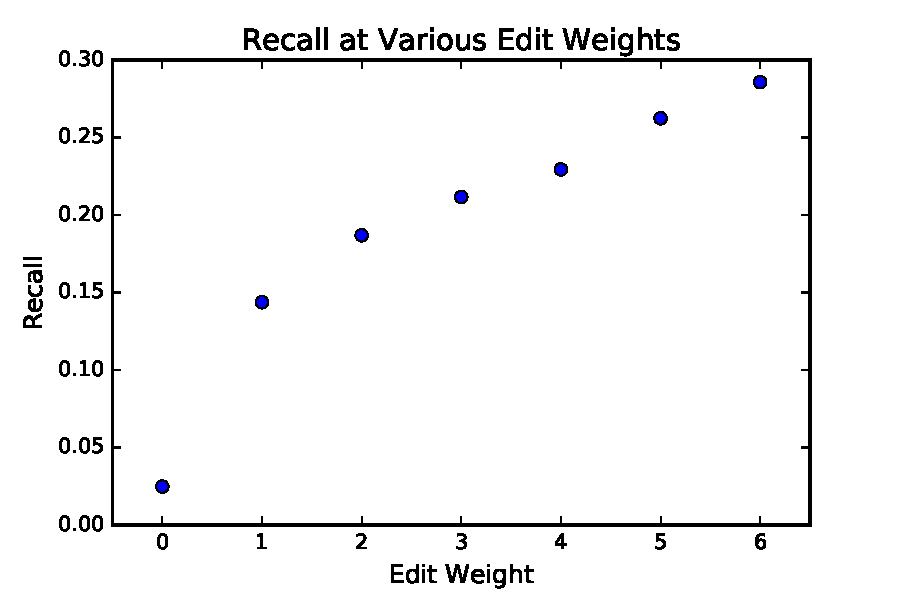
\includegraphics[]{edit_weight_recall}
\caption{The greater the edit weight, the greater the recall.}
\label{fig:edit-weight-recall}
\end{figure}

\begin{figure}[h]
\centering
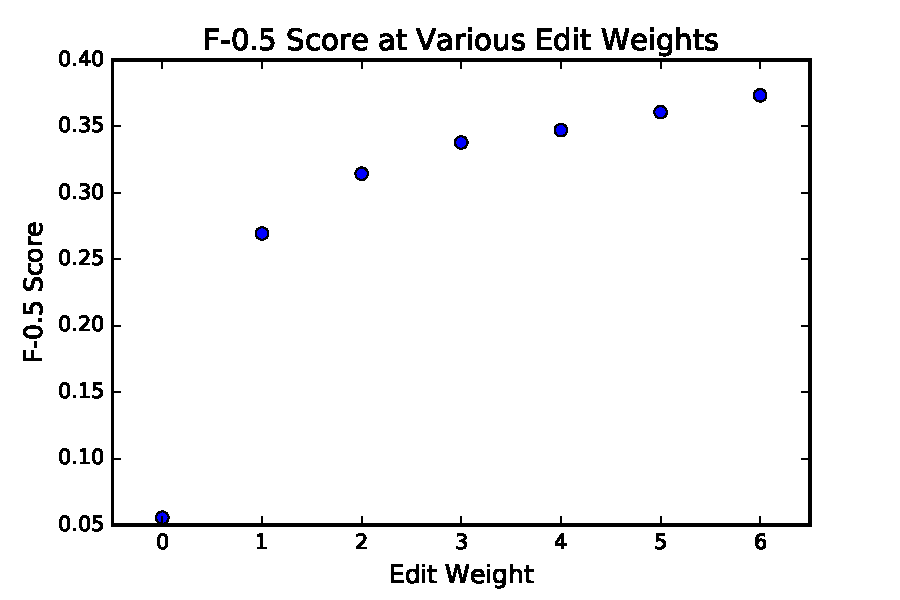
\includegraphics[]{edit_weight_F-0_5}
\caption{Generally speaking, $F_{0.5}$ score also increases with edit weight.}
\label{fig:edit-weight-m2}
\end{figure}